\section{Modified Auxilary Construction.}

Recall that in Theorem \ref{thm:hinge2} we want to show that it is strongly NP-hard to decide whether a polygonal linkage whose hinge graph is a tree can be realized with counter-clockwise orientation.
We modify the auxiliary construction allowing all polygons to move freely, and by adding extra polygons and hinges so that the hinge graph becomes a \emph{tree}, and the size of the construction remains polynomial. 
The auxiliary construction is based on a polynomial sized area of the hexagonal grid, using obstacle hexagons of side lengths $N(n,m)$, unit hexagons (of side length 1), and small hexagons of side length $\frac{1}{3}$. 
We modify it in five steps as follows:

\begin{enumerate}
\item Move the obstacle hexagons apart such that the width of each corridor increases from $\sqrt{3}$ to $\sqrt{3}+1/(100N)$.
\item Replace the unit segment in each clause gadget by a skinny rhombus of diameter $\sqrt{1 + \lr{100N}^{-2}}$ and width $1/(200N)$.
\item Enclose the regular hexagon region $J$ containing all gadgets by a \emph{frame} of 6 congruent regular hexagons, as shown in Fig.~\ref{fig:frame}(a), hinged together in a path. Hinge adjacent frame hexagons at the modpoint of the common side.
\item Connect the frame and the obstacles in $J$ into a simply connected polygonal linkage: in each obstacle
hexagon, the bottom side is adjacent to the frame or to a corridor.
Introduce a hinge at the midpoint of one such side in each obstacle hexagon.
\begin{itemize}
	\item[(a)] If this side is adjacent to the frame, then attach the hinge to the frame. 
	\item[(b)] The hinge is attached to a new \emph{connector} polygon: a skinny rhombus of diameter 1 and width $\frac{1}{200N}$.
	\item[(c)] The far corner of each rhombus is hinged to the unit hexagon in the middle of the corridor at shown in Figure \ref{fig:frame}(b).
\end{itemize} 
\item The construction so far constains rows and columns of obstacle hexagons.
Every other column of obstacle hexagons is hinged to the bottom side of the perimiter of $J$.

\begin{minipage}{\linewidth}
\begin{center}
\includegraphics[width=.9\columnwidth]{graphics/modifiedAuxilaryConstructionAsTree.pdf}
\captionof{figure}{(a) illustrates a tree corresponding to the modified auxilary construction in (b).  On the left half of the tree, we have the bottom most frame hexagons and the the hexagons in the interior of $J$ as children of the the bottom frame hexagons.  The top most frame hexagons only have the half sized hexgons attached to them. (b) is the corresponding modified auxilary construction.}\label{fig:modifiedAuxilaryConstructionAsTree.pdf}
\end{center}
\end{minipage}

These bottom most obstacle hexagons have a hinge point on its side.
The columns that do not have an obstacle hexagon hinged to the perimeter of $J$ has a half-sized hexgon hinged to the perimeter of $J$ and a locked flag with no state to the first obstacle hexagon above it (See Figure \ref{fig:HalfSizeHexagon.pdf}).  
The half-sized hexagon serve to attach free obstacle hexagons to the bottom side of the frame.

\begin{minipage}{\linewidth}
\begin{center}
\includegraphics[width=.33\columnwidth]{graphics/HalfSizeHexagon.pdf}
\captionof{figure}{In this figure we illustrate the bottom of the perimeter of $J$ with three obstacle hexagons, a half sized hexagon, and a locked flag whose hinge points lock the flag's state (becoming stateless).}\label{fig:HalfSizeHexagon.pdf}
\end{center}
\end{minipage}
\end{enumerate}

We obtain a simply connected polygonal linkage. 
We now allow the obstacle hexagons to move freely, and call their original fixed position \emph{canonical}. 
This complests the description of the modified auxiliary construction.  

We may assume without loss of generality that the frame is at its original position. 
It is enough to show that the obstacle hexagons are still confined to an $\frac{1}{s^\kappa}$-neighborhood of their canonical position, then it follows that the polygonal linkage is realizable if and only if $\Phi$ is satisfiable.

\begin{minipage}{\linewidth}
	\begin{center}
	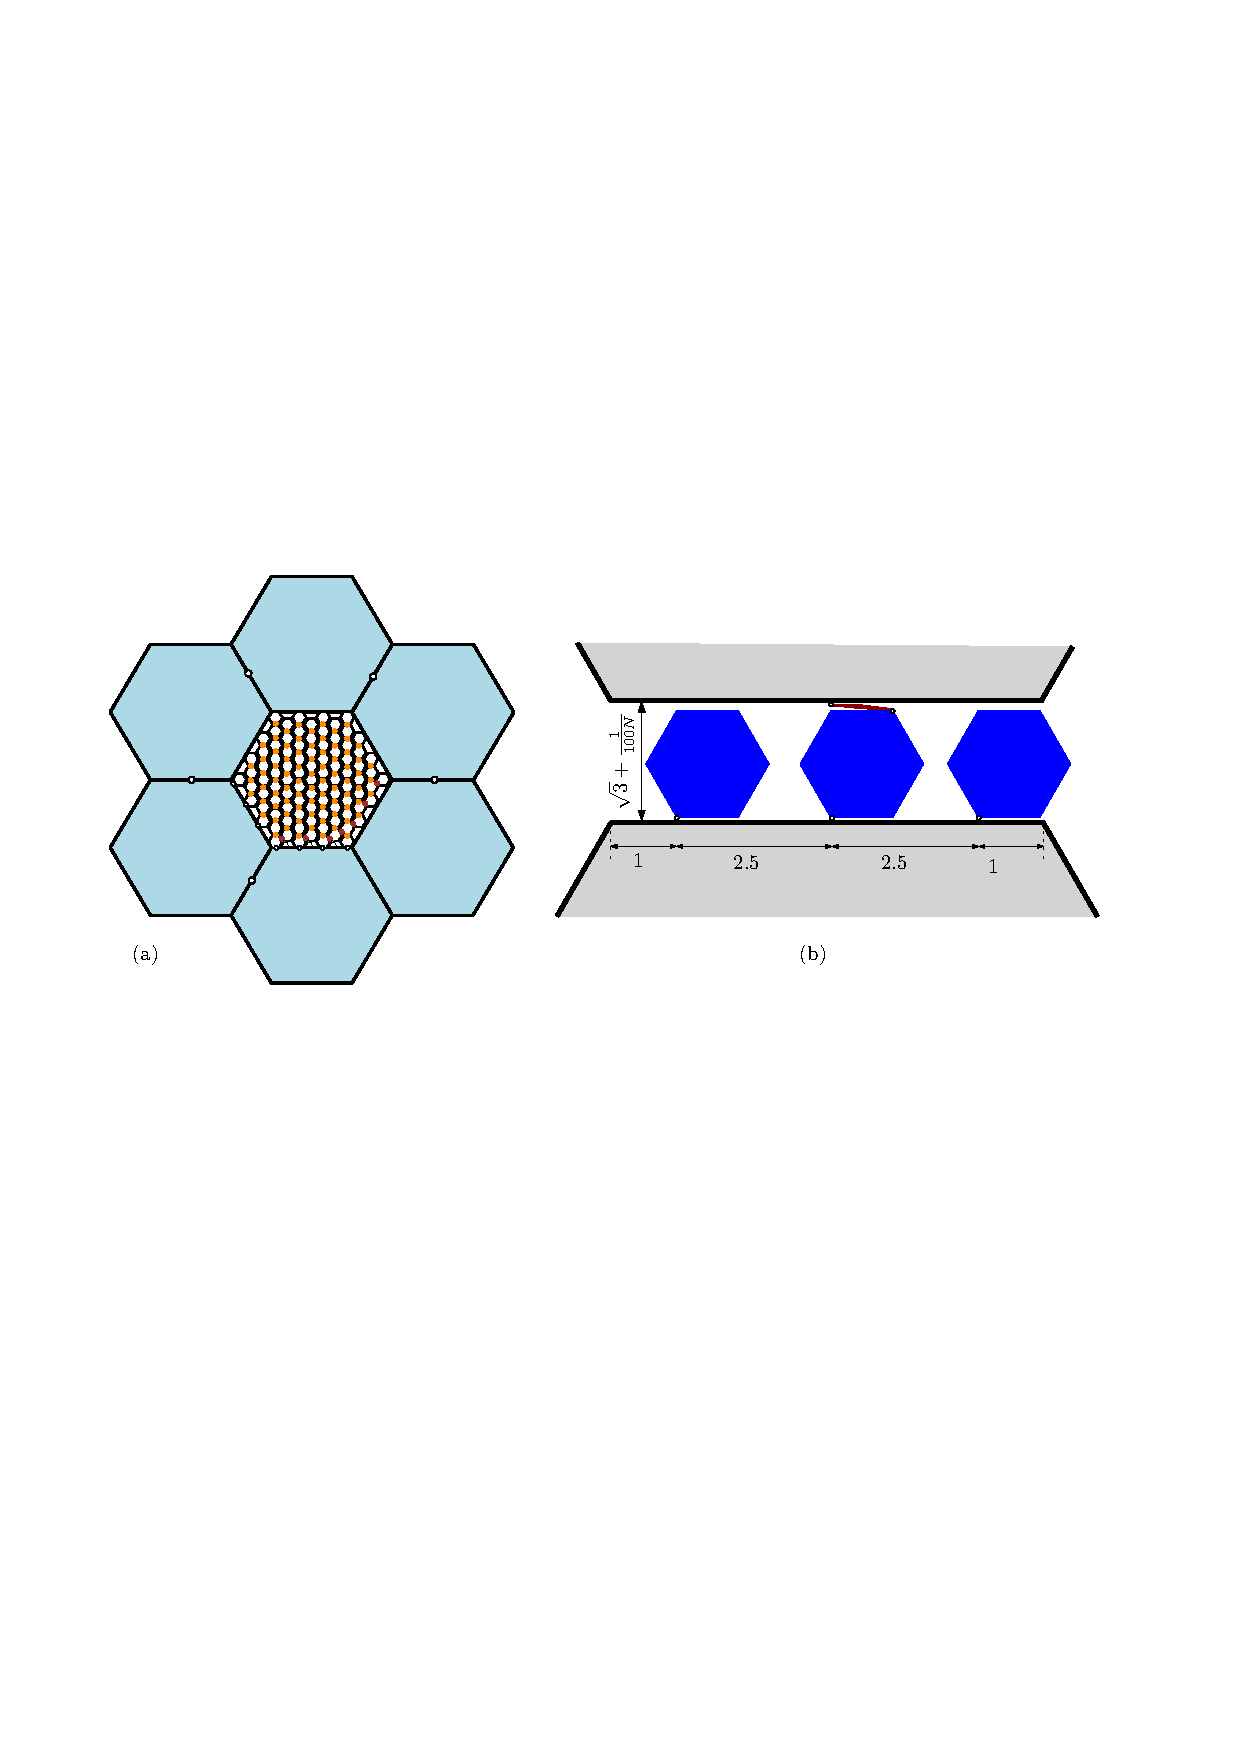
\includegraphics[width=0.95\columnwidth]{graphics/fig-frame-hex}
	\captionof{figure}{(a) A frame (built of 6 hinged regular hexagons) encloses a hexagonal tiling, and
    vertical paths connect all obstacle hexagons to the frame.
    (b) A corridor is widened to $\sqrt{3}+\frac{1}{N^2}$. A connection between
    two adjacent obstacle hexagons is established via a skinny rhombus.}
	\label{fig:frame}
	\end{center}
\end{minipage}

For the remainder of this chapter, suppose there exists a realization, the position of each hexagon can be defined by the isometry from its canonical position; an isometry is given by the triple $\lr{\alpha, \beta, \delta}$ where $\alpha$ is a counter clockwise rotation about the center of the hexagon and $\lr{\beta,\delta}$ is a translation vector.  
Canonical position would have each obstacle hexagon's position as $(0,0,0)$.
